\documentclass{curriculum_vitae}

\begin{document}

\fontfamily{ppl}\selectfont

\noindent
\begin{tabularx}{\linewidth}{@{}m{1\textwidth} m{0\textwidth}@{}}
{
    \Large{Jacek G. Pardyak} \newline
    \small{
        \href{mailto:}{\tt \href{mailto:jacek.pardyak@gmail.com}{\nolinkurl{jacek.pardyak@gmail.com}}}
        \textbf{·} 
            \href{http://jacekpardyak.github.io}{\tt jacekpardyak.github.io} 
        \textbf{·}   
        {\fontdimen2\font=0.75ex 06 X078X34X} 
        \textbf{·}   
         {\fontdimen2\font=0.75ex 2523 YZ 's-Gravenhage}
        \newline
        \frcontent{Software Developer (Python \& R)}{}{}{}
}}
& 
{
    \hfill
}
\end{tabularx}

\begin{center}


\begin{tabularx}{\linewidth}{@{}*{2}{X}@{}}
% left side %
{
    \csection{WORK EXPERIENCE}{\small
        \begin{itemize}

                        
             \item \frcontent{Atos Nederland B.V. }{Data
Scientist - Amstelveen, Netherlands}{Provided consulting services for
industries such as: metallurgy, aviation, railways, retail, telco,
health in the field of data science. Performed descriptive and
predictive analysis of structured and unstructured data in R and Python.
Created dashboards in Shiny and QlikView. Determined the state of
equipment in use (tram and train tracks, aircraft) to predict when
maintenance is due. Conducted customer behavioral segmentation and
social media text sentiment analysis. Build models to recommend the next
best offer, detect never paying or churning customers.}{Mar 2015 - Mar
2021}

            
             \item \frcontent{The National Centre for Research and
Development }{Team leader system development - Warsaw,
Poland}{Documentation of the process flow (process maps, procedures),
development of the Document Management System. Motivating and supporting
5 subordinates.}{Aug 2008 - Feb 2015}

            
             \item \frcontent{Graham Packaging }{Production
planner - Warsaw, Poland}{Plan and analyze results of mold production
for plastic and other metal parts. Programming of CNC machines and
execution of tasks related to the digital transformation of the
organization.}{Apr 1998 - Jul 2008}


      \end{itemize}
    }
%----------------------------------    
    \csection{EDUCATION}{\small
        \begin{itemize}
                        \item \frcontent{Master of Science in
Mathematics}{Maria Curie-Skłodowska University, Lublin Poland}{}{2001}
                    \end{itemize}
    }
%----------------------------------        
\csection{DRIVING LICENSES}{\small
\vspace{0.1cm}
\begin{tabularx}{\linewidth}{@{}*{4}{>{\centering\arraybackslash}X}@{}}
{\centering
{\footnotesize B} 
\includegraphics[width=1.4cm]{images/licenses/license-B.pdf} 
} 
{\centering
{\footnotesize A} 
\includegraphics[width=1.4cm]{images/licenses/license-A.pdf} 
} 
{\centering
{\footnotesize AM} 
\includegraphics[width=1.4cm]{images/licenses/license-AM.pdf} 
} 
{\centering
{\footnotesize T} 
\includegraphics[width=1.4cm]{images/licenses/license-T.pdf} 
} 
 \\
\end{tabularx}
}  

        
} 
% end left side %
& 
% right side %
{

%----------------------------------    
\csection{LANGUAGES}{\small
\begin{tabularx}{\linewidth}{@{}*{3}{>{\centering\arraybackslash}X}@{}}
{\centering \textbf{Language}} & {\centering \textbf{Oral}} & {\centering \textbf{Written}} \\
 
\footnotesize Polish & \footnotesize Excellent & \footnotesize Excellent \\
 
\footnotesize English & \footnotesize Excellent & \footnotesize Excellent \\
 
\footnotesize Dutch & \footnotesize Reasonable & \footnotesize Good \\
 
\footnotesize Russian & \footnotesize Good & \footnotesize Good \\

\end{tabularx}
}

%----------------------------------    
\csection{COMPETENCES}{\small
        \begin{itemize}
        \item { \textbf{Be reliable and honest} \footnotesize The
statement that something is not true also provides knowledge.}
        \item { \textbf{Think logically} \footnotesize I create my own
models of reality to navigate in it.}
        \item { \textbf{Learn} \footnotesize I enjoy learning new
Information Technologies, Data Science algorithms and improved
programming libraries.}
        \item { \textbf{Discover and explore} \footnotesize I like to
discover the secrets hidden in the data.}
        \item { \textbf{Writing and reporting} \footnotesize I like to
share my discoveries with others, so that they gain in value.}
        \end{itemize}
    }      

%----------------------------------    
    \csection{OTHER HIGHLIGHTS}{\small
        \begin{itemize}
        \item \frcontent{What are the Dutch singing
about?  \href{http://jacekpardyak.github.io/Liedboek}{\tt [boek]} }{R
Book with translations of the Dutch lyrics to Polish.}{}{R, R Markdown,
\LaTeX, HTML, ePUB}
        \item \frcontent{Resume  \href{http://jacekpardyak.github.io/resume}{\tt [jacekpardyak.github.io/resume]} }{R
Library for authoring Résumés, CVs and Letters.}{}{R, R Markdown,
\LaTeX}
        \item \frcontent{Kaggle
tutorials  \href{http://www.kaggle.com/jacekpardyak}{\tt [www.kaggle.com]} }{R
Tidyverse and Python TensorFlow applications in the analysis of the
Dutch language and processes taking place in the Netherlands.}{}{R,
Python}
 \end{itemize}
    }

%----------------------------------        
    \csection{INTERESTS}{\small
        \vspace{0.32cm}
        \begin{tabularx}{\linewidth}{@{}*{4}{>{\centering\arraybackslash}X}@{}}
{\centering
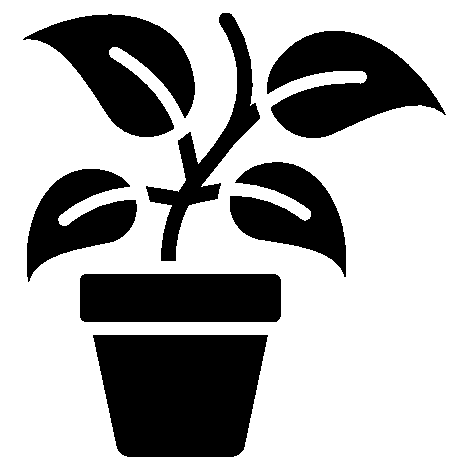
\includegraphics[width=0.8cm]{images/interests/plants.pdf} 
}& 
{\centering

\includegraphics[width=0.8cm]{images/interests/swimming.pdf} 
}& 
{\centering

\includegraphics[width=0.8cm]{images/interests/knitting.pdf} 
}& 
{\centering

\includegraphics[width=0.8cm]{images/interests/diversity.pdf} 
} 
 \\

{\footnotesize Garden \& plants} & 
{\footnotesize Leisure time outdoors} & 
{\footnotesize Programming in R \& Py} & 
{\footnotesize Diversity \& inclusion}  
    \end{tabularx}
    }
% end right side
}
\end{tabularx}
\end{center}
\end{document}